\documentclass[11pt]{article}
\usepackage{fullpage}
\usepackage{setspace}
\usepackage{amsmath}
\usepackage{array}
\usepackage{fancyvrb}
\usepackage{enumerate}
\usepackage{pgfplots}
\usepackage{graphicx}
\usepackage{float}
\usepackage{multirow}
\newcolumntype{L}{>$l<$}
\newcolumntype{R}{>$r<$}

\begin{document}
\noindent\large{Math 5365}\\
\large{Data Mining 1}\\
\large{Homework 5}\\
\large{Mary Barker}
\newline
\doublespace
The code used to solve each question is attached at the end of the document. 

\begin{enumerate}
\item Create a function called splitdata that splits data into training and test sets.\\
See attached r script.

\item Download the file wdbc.data from the Breast Cancer Wisconsin (Diagnostic) 
data set on the UCI machine learning respository. Give a general description of the 
data, and determine what columns 1, 2, 3, 16, and 26 of this data represent.\\
wdbc contains a lits of attibutes for a total of 569 patients. There are 32 
attributes which are the headers of columns. These are as follows: 
\begin{enumerate}
\item Column 1 is the patient ID number.
\item Column 2 is the diagnosis (M or B for Malignant or Benign respectively. 
\item Columns 3-32 give statistics for 10 features of the cells. 
the statistics are mean, standard error and worst mean, which is the mean of the 
3 largest values. The features are: \\
$
\begin{array}{LRl}
radius & columns & 3-5\\
texture & columns & 6-8\\
perimeter & columns & 9-11\\
area & columns & 12-14\\
smoothness & columns & 15-17\\
compactness & columns & 18-20\\
concavity & columns & 21-23\\
concave points & columns & 24-26\\
symmetry & columns & 27-29\\
fractal dimension & columns & 30-32
\end{array}
$

Column 3 contains mean radius, column 16 contains standard error of smoothness, and 
column 26 contains worst mean of concave points.
\end{enumerate}
\item 
\begin{enumerate}
\item Now that we know what column 1 is, we know that we don't want any algorithm 
using this column to make predictions, so remove it from the data.\\

\begin{Verbatim}
wdbc <- wdbc[ -c(1) ]
\end{Verbatim}

\item Use splitdata to split the data into 70\% training and 30\% test data. \\

\begin{Verbatim}
splitlist <- splitdata(wdbc, 0.7, FALSE)
traindata <- splitlist$traindata
testdata <- splitlist$testdata
\end{Verbatim}

\item Find colSums and dim of the original data and of the training and test data to verify 
that the splitting was done correctly. \\

\begin{Verbatim}
tot_sum = as.numeric(colSums(wdbc[,-1]))
sum1 = as.numeric(colSums(traindata[,-1]))
sum2 = as.numeric(colSums(testdata[,-1]))
newsum = sum1+sum2
if(sum(tot_sum - newsum) >= 0.5){ # because of roundoff error they
  print(sum(tot_sum - newsum))    # will only be approximately equal
  print("error: traindata and testdata don't divide whole dataset")
}
\end{Verbatim}

The split was done correctly according to the test shown above. 
In order to check that the number of rows in traindata and testdata add up to the 
total number of rows in wdbc, dim() was used. The results are as follows. \\

\begin{Verbatim}
> dim(wdbc)
569 31
> dim(traindata)
398 31
> dim(testdata) 
171 31
\end{Verbatim}

Since 70\% of 569 is approximately 398, the splitdata function not only subdivides the 
data into training and testing data so that they partition the original set, but it 
does so with the correct distribution as well. 
\end{enumerate}
\item 
\begin{enumerate}
\item Use rpart to fit a tree called tree1 to this data, plot it, and calculate its 
training and test error rates. \\
The commands used to create the tree are in the script at the end of this document. 

\begin{center}
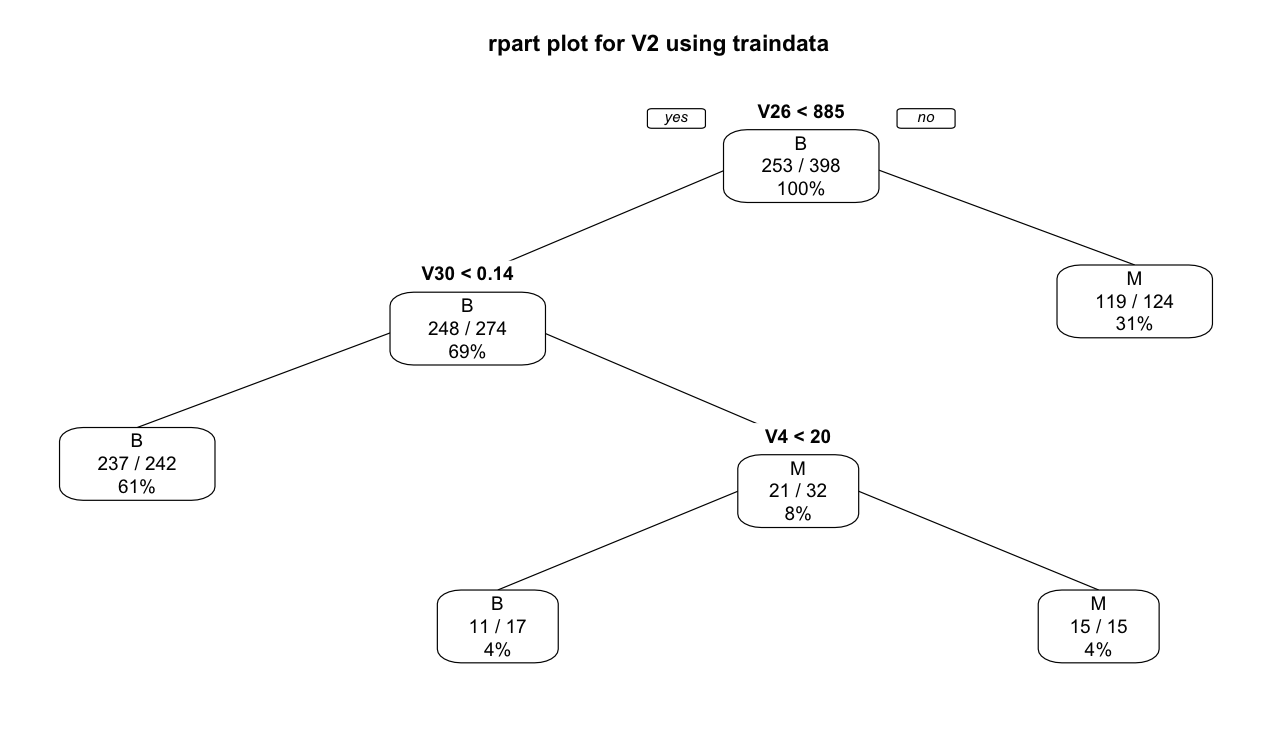
\includegraphics[scale=0.25]{rpartplot_1}
\end{center}
The tree had a train error of 0.04020101 and a test error of 0.05263158.

\item Use ctree to fit a tree called tree2 to this data, plot it, and calculate its 
training and test error rates. \\

\begin{center}
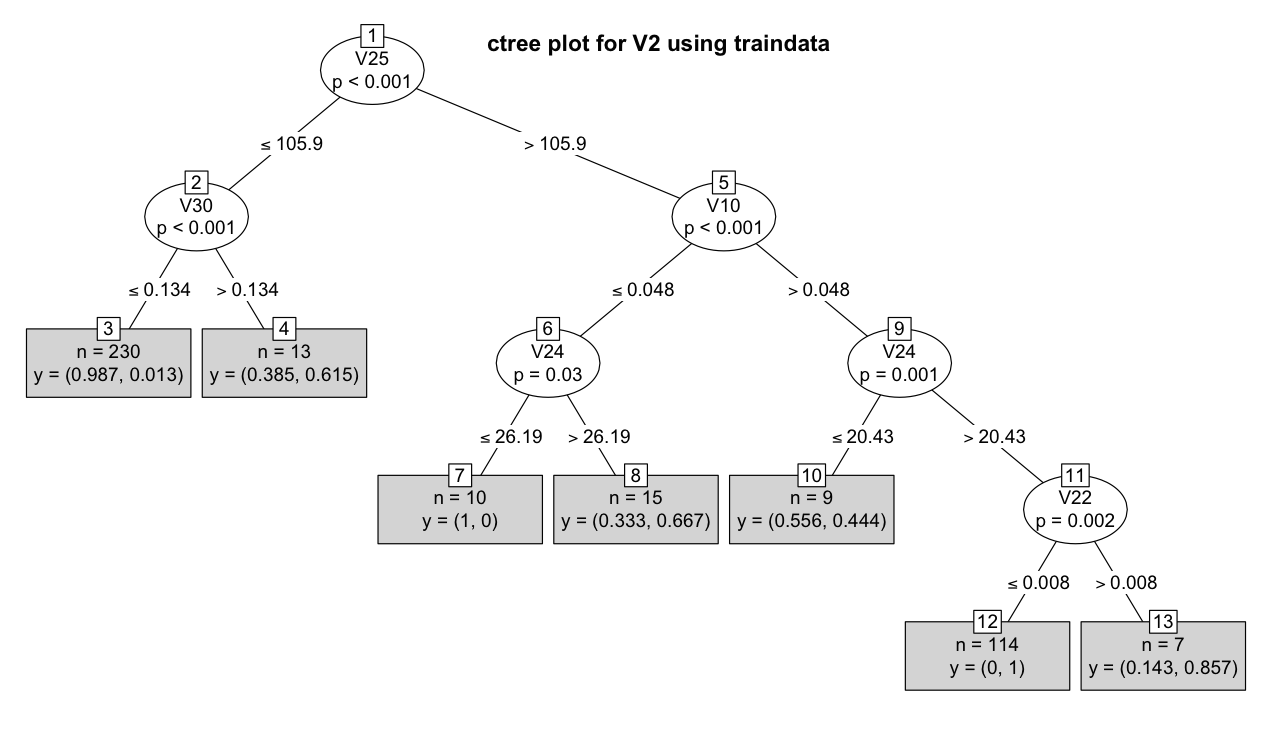
\includegraphics[scale=0.25]{ctreeplot_1}
\end{center}
The tree had a train error of 0.04522613 and a test error of 0.0877193.

\item Intuitively, dose there appear to be a statistically significant difference between
the accuracies of tree1 and tree2 ? \\

No.  The training error is practically the same for one run at least, and 
 the testing error is only slightly higher for ctree. 

\item Test whether the difference in accuracies is statistically significant. \\
Using McNemar's test with the two trees gave a $p-$ value of 0.2379, which is not 
small enough to demonstrate a significant difference between the two trees. 

\end{enumerate}
\item Estimate the accuracy of ctree using the following types of cross validation. \\

\begin{enumerate}
\item 10-fold cross-validation.\\
Using 10-fold cross-validataion gave an average error estimate of 0.06325188.
\item 20-fold cross-validation. \\
Using 20-fold cross-validataion gave an average error estimate of 0.07354041.
\item Leave-one-out cross-validation. \\
Using Leave-one-out cross-validataion gave an average error 
estimate of 0.07732865.
\item Delete-d cross-validation with d = 20, m = 100.\\
Using Delete-d cross-validataion gave an average error estimate of  0.083.
\item the bootstrap with b = 100.\\
The Bootstrap method gave an average error of 0.03057996.
\end{enumerate}
\end{enumerate}
\singlespace
\begin{Verbatim}
#Data Mining Hw 5
#Most of the functionality in here is generalized in file ../dataset_ops.R

#1) Create a function called splitdata that splits data into 
#   training and test sets
splitdata = function(data, trainfrac, rep){
	if((trainfrac > 1) | (trainfrac < 0)){
		print("error in function splitdata: trainfrac not in [0 1]")
	}

	tot_size = nrow(data)
	train_list = sample(tot_size, round(trainfrac * tot_size, digits=0), 
	                    replace = rep)
	traindata <- data[train_list, ]
	testdata <- data[-train_list, ]
	mylist <- list(traindata = traindata, 
                       testdata = testdata, train = train_list)
    return(mylist)
}
#splitlist <- splitdata(iris, 0.7, FALSE)

#2) Download the file wdbc.data from the Breast Cancer Wisconsin (Diagnostic)
#   data set on the UCI Machine Learning Repository. Give a general 
#   description of the data, and determine what columns 1, 2, 3, 16, and 26 
#   of this data represent.

wdbc <- read.table("~/Dropbox/Tarleton/data_mining/hw05/wdbc.data",
header=FALSE,sep=",")

if(FALSE){
  wdbc contains a list of attributes for a total of 569 patients.
  There are 32 attributes(in columns)
  Column 1 is the patient ID number
  Column 2 is Diagnosis(M or B for Malignant or Benign respectively)

  Columns 3-32 gives statistics for 10 features of the cells. 
  The statistics are mean, standard error and mean of the 3 largest values 

  The features are : 
 1 radius              columns 3-5
 2 texture             columns 6-8
 3 perimeter           columns 9-11
 4 area                columns 12-14
 5 smoothness          columns 15-17
 6 compactness         columns 18-20
 7 concavity           columns 21-23
 8 concave points      columns 24-26
 9 symmetry            columns 27-29
 10 fractal dimension  columns 30-32

 Column 3  contains mean radius
 Column 16 contains standard error of smoothness
 Column 26 contains mean of the 3 largest values of concave points
}

#3) 
##a. Now that we know what column 1 is, we know that we don't want any 
##   algorithm using this column to make predictions, so remove it from 
##   the data. 
wdbc <- wdbc[ -c(1) ]
##b. Use splitdata to split the data into 70% training and 30% test data. 
splitlist <-splitdata(wdbc, 0.7, FALSE)
traindata <- splitlist$traindata
testdata <- splitlist$testdata
train <- splitlist$train

##c. Find colSums and dim of the original data and of the training and test 
##   data to verify that the splitting was done correctly.

tot_sum = as.numeric(colSums(wdbc[,-1]))
sum1 = as.numeric(colSums(traindata[,-1]))
sum2 = as.numeric(colSums(testdata[,-1]))
newsum = sum1 + sum2

if(sum(tot_sum - newsum) >= 0.5){ # because of roundoff error they
  print(sum(tot_sum - newsum))    # will only be approximately equal
  print("error: traindata and testdata don't divide whole dataset")
}

dim(wdbc)
#569  31
dim(traindata)
#398  31
dim(testdata)
#171  31

#4) 
##a. Use rpart to fit a tree called tree1 to this data, plot it, and 
##   calculate its training and test error rates.
library(rpart)
library(rpart.plot)
library(treemap)

tree1 = rpart(V2~., traindata)
p_tree1_train = predict(tree1, traindata,type='class')
prp(tree1, type=1, extra=102)
title("rpart plot for V2 using traindata")
m_tree1 = table(traindata$V2, p_tree1_train)
train_error1 = 1 - (sum(diag(m_tree1)) / sum(m_tree1))

p_tree1_test = predict(tree1, testdata, type = 'class')
m_tree1 = table(testdata$V2, p_tree1_test)
test_error1 = 1 - (sum(diag(m_tree1)) / sum(m_tree1))

##b. Use ctree to fit a tree called tree2 to this data, plot it, and 
##   calculate its training and test error rates.
library(party)

tree2 = ctree(V2~., traindata)
plot(tree2, type='simple')
title("ctree plot for V2 using traindata")

p_tree2_train = predict(tree2, traindata)
m_tree2 = table(traindata$V2, p_tree2_train)
train_error2 = 1 - (sum(diag(m_tree2)) / sum(m_tree2))

p_tree2_test = predict(tree2, testdata)
m_tree2 = table(testdata$V2, p_tree2_test)
test_error2 = 1 - (sum(diag(m_tree2)) / sum(m_tree2))

##c. Intuitively, does there appear to be a statistically significant 
##   difference between the accuracies of tree1 and tree2? 

# No. The training error is practically the same for one run at least, and 
# the testing error is only slightly higher for ctree. 

##d. Test whether the difference in accuracies is statistically significant. 

library(stats)
library(exact2x2)
library(exactci)
accvector1 = (testdata$V2 == predict(tree1, testdata, type= 'class'))
accvector2 = (testdata$V2 == predict(tree2, testdata))

mcnemartable=table(accvector1, accvector2)

mcnemar.exact(mcnemartable)

#5) Estimate the accuracy of ctree using the following types 
#   of cross validation. 

kfold_val = function(k, treetype, wdbc){
	total_acc = 0
	size = ceiling(nrow(wdbc)/k)
    folds = sample(rep(1:k,size))
    myvec = folds[1:nrow(wdbc)]

	for(i in 1:k){

        testdata <- wdbc[myvec==i,]

        traindata <- wdbc[myvec!=i,]
        print(nrow(traindata))
        if(treetype == 0){
            mynewtree = ctree(V2~., traindata)
        } else if(treetype == 1){
            mynewtree = rpart(V2~., traindata)
        }

        p_tree_train <- predict(mynewtree, testdata)
        
        m_tree = table(testdata$V2, p_tree_train)
        test_acc = (sum(diag(m_tree)) / sum(m_tree))
        total_acc = total_acc + test_acc
	}
	total_acc = total_acc / k
	return(1 - total_acc)
}

##a. 10-fold cross-validation
error10 = kfold_val(10, 0, wdbc)

##b. 20-fold cross-validation
error20 = kfold_val(20, 0, wdbc)

##c. Leave-one-out cross-validation
error_leave_one_out = kfold_val(nrow(wdbc), 0, wdbc)

##d. Delete-d cross-validataion with d = 20 and m = 100.
delete_d_cv = function(m, d, mytree, wdbc){
  total_acc = 0
  for(i in 1:m){
     splitlist <- splitdata(wdbc, 1 - d / nrow(wdbc), FALSE)
     traindata <- splitlist$traindata
     testdata <- splitlist$testdata
     if(mytree < 1){
       mynewtree = ctree(V2~., traindata)
     }else{
       mynewtree = rpart(V2~., traindata, type='class')
     }

     p_tree_train <- predict(mynewtree, testdata)

     m_tree = table(testdata$V2, p_tree_train)
     test_acc = (sum(diag(m_tree)) / sum(m_tree))
     total_acc = total_acc + test_acc
   }
   total_acc = total_acc / m
   return(1 - total_acc)
}
deletedcv = delete_d_cv(100, 20, 0, wdbc)

##e. The bootstrap with b = 100

bootstrap = function(b, mytree, wdbc){
    total_acc = 0
    n = nrow(wdbc)
    for(i in 1:b){
         splitlist <- splitdata(wdbc, 1, TRUE)
         traindata <- splitlist$traindata
         testdata <- splitlist$traindata
      	 if(mytree < 1){
           mynewtree = ctree(V2~., traindata)
      	 }else{
           mynewtree = rpart(V2~., traindata)	
      	 }
         p_tree_train <- predict(mynewtree, testdata)
         m_tree = table(testdata$V2, p_tree_train)
         test_acc = sum(diag(m_tree)) / sum(m_tree)
         total_acc = total_acc + test_acc
    }
    total_acc = total_acc / b
    return(1 - total_acc)
}
b1 = bootstrap(100, 0, wdbc)
\end{Verbatim}


\end{document}
